\section{重整化}
在QFT中我们经常遇到某些量发散的情况, 为了解决这个问题, 我们引入重整化步骤, 将无穷大扫到地板下, 从而得到有限的可观测量预测.
\subsection{Casmir效应}
在\ref{2nd_quant_free_real_scalar}节中, 我们得知, 自由实标量场的真空零点能是无穷大. 不过这并不影响我们的物理实际, 因为能量并不是一个直接可观测量: 能量的差值才是, 比如说受力. 这就是Casmir效应: 在真空中的两块板之间, 由于板的存在产生的边界条件, 真空模态被改变, 导致两块板之间的能量密度与外部不同, 从而产生一个可观测的吸引力. 

\begin{figure}[!htbp]
    \centering
    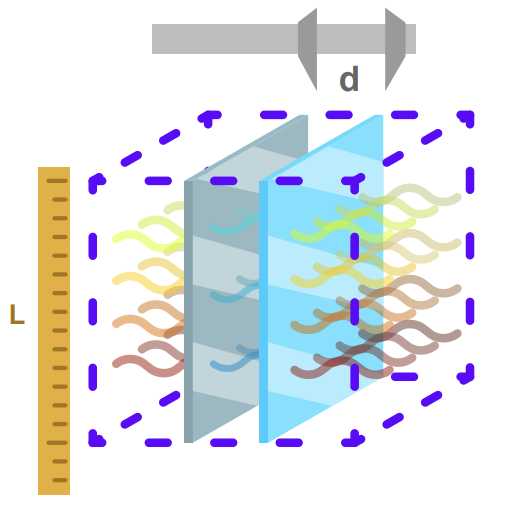
\includegraphics[width=0.4\textwidth]{./image/casmir.png}
    \caption{Casmir效应示意图}
    \label{fig:casmir}
\end{figure}

为了简单起见我们首先考虑一维的情况, 假设两板的距离为$a$. 边界条件要求
\begin{align}
    \begin{cases}
        \phi(0,t)=0\\
        \phi(a,t)=0,
    \end{cases}
\end{align}
这要求波矢满足
\begin{equation}
    \vec k\cdot L\vec n=\vec p\cdot d\vec n=p_x d=n\pi
\end{equation}
于是
\begin{equation}
    k=\frac{n\pi}{a}.
\end{equation}

从而求出总能量
\begin{align}
    E(a)=\sum_{n=0}^{+\infty}\frac12\frac{n\pi}{a}=\frac{\pi}{2a}\sum_{n=0}^{+\infty}n.
\end{align}

这个求和显然是发散的, 发散的原因是我们直接将波矢推到了无穷远处的紫外区, 但是这一假设实际上是有问题的, 因为当波长到原子量级, 我们必须考虑它和极板之间的互相作用, 这样子自由场论也不适用了. 但是我们可以断定, 一个紫外完备的合适理论一定可以让高动量的贡献是被抑制的, 因此紫外的贡献实际上是可以被忽略掉的. 于是我们可以人为引入一个很高的截断动量$\Lambda$, 并让求和在此处截断:
\begin{align}
    n_{\rm{max}}=\lfloor a\Lambda \rfloor.
\end{align}
这等价于给求和乘了一个核函数
\begin{align}
    f(x)=\Theta(n_{\rm{max}}-r\Lambda x),
\end{align}
\begin{align}
    E(a)=\frac{\pi}{2a}\sum_{n=0}^{+\infty}nf(\frac{n}{r \Lambda}).
\end{align}
当然, 也可以有其他的核函数取法(一个更详尽的核函数距离可以见Schwartz\cite{schwartz-kernel}), 比如指数衰减:
\begin{align}
    f(x)=\exp{-x}, 
\end{align}
这称为热核函数.

不过需要注意, 这只是两板之间的真空能, 我们应当把两板外侧的真空能一起算入. 在这里我们认为左侧板固定, 右侧板可以移动, 因此左侧板左侧的真空能量是常数, 我们可以不计入. 而为了方便计算右侧板上真空能的大小, 我们不妨在右侧板$L\gg a$出再引入一个极板, 来方便我们估计右侧的真空能, 从而有

\begin{align}
    E_{\rm{tol}}(a)=E(a)+E(L-a)
\end{align}

由于$L\gg a$, 我们可以做连续化近似, 将求和化为积分:
\begin{align}
    E(L-a)&=\frac{\pi}{2(L-a)}\sum_{n=0}^{+\infty}nf(\frac{n}{(L-a)\Lambda})\\
    &=\frac\pi2(L-a)\Lambda^2\sum\frac1{(L-a)\Lambda}\frac{n}{r\Lambda}f(\frac{n}{(L-a)\Lambda})\\
    &=\frac\pi2\Lambda^2(L-a)\int_0^{+\infty}\d xxf(x).
\end{align}

丢掉常数项, 我们可以得到总能量
\begin{align}
    E_{\rm{tot}}(a)&=-\frac\pi2\Lambda^2a\int_0^{+\infty}\d xxf(x)+\frac{\pi}{2a}\sum_{n=0}^{+\infty}nf(\frac{n}{r \Lambda})
\end{align}
再对积分做换元
\begin{align}
    x=\frac{n}{a\Lambda}
\end{align}
从而有
\begin{align}
    E_{\rm{tot}}(a)&=\frac{\pi}{2a}\left(\sum nf(\frac n{a\Lambda})-\int\d nnf(\frac n{a\Lambda})\right).
\end{align}

根据Euler-Maclaurin公式
\begin{align}
    \sum_{n=1}^NF(n)-\int_0^N\d n F(n)&=\frac{F(0)+F(N)}2+\frac{F'(N)-F'(0)}{12}\notag\\
    &\;\;-\frac1{30}\frac{F^{(3)}(N)-F^{(3)}(0)}{4!}+\cdots+B_j\frac{F^{(j-1)}(N)-F^{(j-1)}(0)}{j!}+\cdots
\end{align}
其中, 对于$j>1$的奇数项, $B_j=0$. 我们可以计算得到一个有限值:
\begin{align}
    E_{\rm{tot}}(a)&=-\frac\pi{24a}, 
\end{align}
从而有受力
\begin{align}
    F(a)=-\de Ea=-\frac\pi{24a^2}. 
\end{align}

类似地, 我们可以计算三维标量场的Casmir效应, 假设极板距离为$a$, 面积为$A$:
\begin{align}
    \frac EA&=\sum_n\int\frac{d^2k}{\dpi2}\frac12\sqrt{\left(\frac{n\pi}a\right)^2+k^2}\\
    &=\frac12\sum_n\int_0^{+\infty}\frac{k\d k}{2\pi}\sqrt{\left(\frac{n\pi}a\right)^2+k^2}.
\end{align}

同样地, 我们引入核函数
\begin{align}
    f(x)=\exp{-x}, 
\end{align}
于是有
\begin{align}
    \frac EA&=\frac12\sum_n\int_0^{+\infty}\frac{k\d k}{2\pi}\sqrt{\left(\frac{n\pi}a\right)^2+k^2}f\left({\sqrt{\left(\frac{n\pi}a\right)^2+k^2}}/\Lambda\right)\\
    &=\frac{\Lambda^3}{4\pi}\sum_n\int_{\frac{n\pi}{\Lambda a}}^{+\infty}u^2\exp{-u}\d u\\
    &=\frac{\Lambda^3}{2\pi}\sum_n\left[1+\frac{n\pi}{\Lambda a}+\frac12\left(\frac{n\pi}{\Lambda a}\right)^2\right]\exp{-\frac{n\pi}{\Lambda a}}.
\end{align}

引入一个$L\gg a$处的极板, 我们有总能量
\begin{align}
    \frac{E_{\rm{tot}}}A&=\frac{\Lambda^3}{2\pi}\left(\sum_n\left[1+\frac{n\pi}{\Lambda a}+\frac12\left(\frac{n\pi}{\Lambda a}\right)^2\right]\exp{-\frac{n\pi}{\Lambda a}}-\int_0^{+\infty}\d n\left[1+\frac{n\pi}{\Lambda a}+\frac12\left(\frac{n\pi}{\Lambda a}\right)^2\right]\exp{-\frac{n\pi}{\Lambda a}}\right).
\end{align}
利用Euler-Maclaurin公式, 我们可以得到一个有限值:
\begin{align}
    \frac{E_{\rm{tot}}}A=-\frac{\pi^2}{1440a^3}.
\end{align}

如果是电磁波, 它有两个极化方向, 因此总能量是标量场的两倍:
\begin{align}
    \frac{E_{\rm{tot}}}A=-\frac{\pi^2}{720a^3}.
\end{align}
从而有受力
\begin{align}
    F=-\de Ea=-\frac{\pi^2}{240a^4}A
\end{align}

\subsection{重整化的一般理论}
为什么量子场论中会出现发散的积分? 其实归根到原因, 我们认为是理论中的量与实际的观测物理量并不匹配导致的: 没有人保证相互作用理论的Lagrangian中的$m, \lambda$就是我们物理观测出来的数. 如果我们胡乱地将物理量直接塞到Lagrangian里, 出现发散的积分是必然的. 但是只要我们做好物理量的匹配工作, 将Lagrangian中的参数与物理观测量进行恰当的匹配, 还是可以消除积分的无穷大的. 

一般地来说, 有三类物理量需要我们进行重新匹配: 质量$m$, 相互作用强度$g$, 还有波函数的归一因子$Z_\phi$. 前两个是直接出现在Lagrangian里的, 而$Z_\phi$似乎是这里凭空出现的, 有点无厘头. 其来源其实是, 我们在使用一般的场量的LSZ公式的时候, 是默认了
\begin{align}
    \braket{p|\phi(x)|0}=\exp{ipx},
\end{align}
这个在自由场中, 我们通过选取恰当的$\a p$是可以轻松满足的. 但是对于相互作用场来说, 
\begin{align}
    \braket{p|\phi(x)|\Omega}=\exp{ipx}
\end{align}
是并不一定能够满足的, 一般地来说有
\begin{align}
    \braket{p|\phi(x)|\Omega}=Z_\phi^{1/2}\exp{ipx}.
\end{align}
这个和我们实验中观测到的场量也不是一个, 也需要一次重新匹配. 所以我们需要将$\phi$进行重新归一化, 也就是
\begin{align}
    \phi(x)=Z_\phi^{1/2}\phi_r(x), 
\end{align}
其中$\phi$是Lagrangian中出现的而$\phi_r(x)$则是实验中测量的. 

不过我们可能会质疑, 场量本身多数时候都不是直接的实验可观测量, 我们将场量与实验观测匹配上是什么意思? 实际上来说, 我们实验中可观测的是场量的两点关联函数$\braket{\Omega|\mathcal T\phi(x)\phi(y)|\Omega}$, 这个可以通过测量相互作用的吸引排斥力(从而得到相互作用势)得到. 

通过这样的重新定义方式, 我们可以得到与实际物理量匹配后的Lagrangian. 比如说对于$\phi^4$理论, 
\begin{align}
    \mathcal L=\frac12(\partial\phi)^2-\frac12m_0^2\phi^2-\frac{\lambda_0}{4!}\phi^4.
\end{align}
我们设
\begin{align}
    Z_\phi=1+\delta_Z, m_0^2Z_\phi=m^2+\delta_m, \lambda_0Z_\phi^2=\lambda+\delta_\lambda,
\end{align}
其中$m^2$是实验测量出的真实物理质量, $\lambda$是某个碰撞条件下实验观测出来的散射振幅(截面), 这被称为on-shell scheme(更具体的要求见下面on-shell scheme的定义). 而$m_0, \lambda_0$则是Lagrangian中的裸参数. 于是我们可以得到
\begin{align}
    \mathcal L=\frac12(\partial\phi_r)^2-\frac12 m^2\phi_r^2-\frac\lambda{4!}\phi_r^4+\frac12\delta_Z(\partial\phi_r)^2-\frac12\delta_m\phi^2-\frac{\delta_\lambda}{4!}\phi_r^4.
\end{align}
其中后面的项被称为反项. 通过恰当地选取反项的值, 我们可以吸收掉计算中的无穷大, 并与实验结果正确地相匹配.

当然, 与真实物理量的匹配并不只这一种方式, 我们后面会看到, 还有其他将物理量与模型相匹配的方式, 不同的匹配方式都是一种方案.
\begin{definition}[方案(Scheme)]
    方案就是指将实验观测的物理量与物理模型匹配的方式.
\end{definition}
我们的微扰计算结果是强烈依赖于方案的, 理论上来说, 只有我们考虑无穷阶的微扰, 才能使得计算结果与方案无关(但是这是做不到的).

\begin{definition}[on-shell方案]
    我们要求, 在on-shell scheme中, 按如下方式匹配反项:
    \begin{itemize}
        \item 模型计算的关联函数极点(这里是指将关联函数视为$f(z), z=p^2$这样一个复变函数)为实验测量的质量$m^2$
        \item 模型计算的关联函数极点处留数为$i$
        \item 模型计算的在阈值时的散射振幅为实验测量的散射振幅.
    \end{itemize}
\end{definition}

\subsubsection{量纲分析}
在量子场论中, 我们经常会遇到发散的圈图, 也就是类似这样的积分
\begin{align}
    \int\dddd p \frac i{p^2-m^2+i\epsilon}.
\end{align}
我们要估算这个积分的发散程度, 可以直接通过量纲来估计: $\dddd p$量纲为$[m]^4$, 传播子贡献$[m]^{-2}$, 故总共$[m]^2$的量纲, 所以我们可以预估它的发散随截断能标是平方发散. 

一般地说, 对于形如
\begin{align}
    \int^{+\infty} p^{D-1}\d p,
\end{align}
的积分, 其发程度为$[\Lambda]^{D}$, $D=0$时为$\ln\Lambda$. 这里$D$即我们想要估算的量纲参数: 表面发散程度(superficial degree of divergence). 但是需要注意, 它并不一定能完全表征图的发散程度: 子图的发散可能会让$D$算出来不发散的图也发散; 规范对称性可能提取出整体的动量使得$D$算出来发散的图实际上不发散. 但是作为一个粗糙的估计也暂时足够了.

做一点量纲分析不难发现, 
\begin{align}
    [x]^d[\mathcal L]=[S]=1, 
\end{align}
这意味着
\begin{align}
    [\mathcal L]=[m]^d.
\end{align}
基于此我们不难得到对于标量场$[\phi]=m^{\Delta_\phi}$, 旋量场$[\psi]=m^{\Delta_\psi}$, 矢量场$[A_\mu]=m^{\Delta_A}$, 有
\begin{align}
    \Delta_\phi=\frac{d-2}2, \Delta_\psi=\frac{d-1}2, \Delta_A=\frac{d-2}2.
\end{align}
这个可以总结为
\begin{align}
    \Delta_f=\frac{d-2}2+S_f,
\end{align}
其中对于Fermi场$S_f=\frac12$, 对于Bose场$S_f=0$. 于是我们还可以知道$f$场的传播子动量量纲为$2\Delta_f$.

然后对于某个相互作用顶点$i$
\begin{align}
    g_i\partial O O\cdots,
\end{align}
若其有$\mathcal D_i$个$\partial$, $N_{if}$个$f$场, 则可知其耦合常数的
\begin{align}
    \Delta_i=d-\mathcal D_i - \sum_f n_{if}\Delta_f.
\end{align}

然后我们可以直接计算内线、相互作用顶点的$\partial$以及动量守恒$\delta^4$带来的总的动量量纲$D$
\begin{align}
    D=\sum_f 2I_f\Delta_f+\sum_i N_i\mathcal D_i-\sum_i dN_i+d.
\end{align}
需要注意, 这里最后$+d$是因为我们算散射振幅的时候要先扣掉一个最后整体的$\delta^4(p)$.

对于一个图来说, 设它有$I_f$个$f$场的内线, $E_f$个$f$场的外线, $N_i$个相互作用顶点$i$, 则我们有拓扑结构(连通图)带来的约束
\begin{align}
    2I_f+E_f=\sum_i N_i n_{if}.
\end{align}
代入此约束条件我们可以化简得到
\begin{align}
    D=d-\sum_f E_f\Delta_f-\sum_i N_i\Delta_i.
\end{align}

然后我们对此式进行简单讨论. 可以看到, 对于$\Delta_i>0$, 保持外脚不变, 相互作用顶点越多$D$越小, 因此在考虑高阶圈图的时候结果将会是收敛的, 这被称为是超重整化的(super renormalizable). 对于$\Delta_i=0$, 收敛性与阶数无关, 但是只有有限个振幅(子图)是UV发散的. 而对于$\Delta_i<0$, 情况就糟糕了: 随着圈数增加, 积分的收敛性越来越差, 这被称为不可重整化的(non-renormalizable). 在后面我们会看到, 为什么说对于$\Delta_i<0$, 理论是不可重整化的.

这里举几个常见例子
\begin{align}
    & \mathcal L_i=\frac\lambda{4!}\phi^4, \Delta_i=0, \textrm{renormalizable in } d=4,\notag\\
    & \mathcal L_i=\frac\lambda{3!}\phi^3, \Delta_i=1, \textrm{super-renormalizable in } d=4,\notag\\
    & \mathcal L_i=\bar\psi\slashed A\psi, \Delta_i=0, \textrm{renormalizable in } d=4,\notag\\
    & \mathcal L_i=G(\bar\psi\psi)^2, \Delta_i=-2, \textrm{non-renormalizable in } d=4,\notag\\
    & \mathcal L_i=\frac\lambda{6!}\phi^6, \Delta_i=-2, \textrm{non-renormalizable in } d=4.\notag
\end{align}

\subsubsection{物理量的匹配}
我们以$\phi^4$理论与on-shell方案为例, 介绍重整化的一般方法. 首先我们引入反项(Counterterm), 得到
\begin{align}
    \mathcal L&=\frac12(\partial\phi_r)^2-\frac12 m^2\phi_r^2-\frac\lambda{4!}\phi_r^4+\frac12\delta_Z(\partial\phi_r)^2-\frac12\delta_m\phi^2-\frac{\delta_\lambda}{4!}\phi_r^4,
\end{align}
其中我们认为反项都是微扰项, 并利用分部积分$\frac12\delta_Z(\partial\phi_r)^2=-\frac12\delta_Z\phi_r\Box\phi_r$, 可以得到反项的顶点
% 这里不用tikz-feynman是实在没招了，不是渲染不出crossed dot就是编译不过...
\begin{align}
    \begin{tikzpicture}[baseline=-0.5ex]
        % 画传播子直线
        \draw[thick] (-1.2, 0) -- (1.2, 0);
        % 在正中间放置计数项符号
        \node[counterterm] at (0, 0) {};
    \end{tikzpicture}
    &= i(p^2 \delta_z - \delta_m), \notag\\
    \begin{tikzpicture}[baseline=-0.5ex]
        % 直接画两条贯穿的对角线（交叉线）
        \draw[thick] (-0.9, -0.9) -- (0.9, 0.9);
        \draw[thick] (-0.9, 0.9) -- (0.9, -0.9);
        % 在中心交点处放上计数项，自动依靠 fill=white 完美遮挡交点
        \node[counterterm] at (0, 0) {};
    \end{tikzpicture}
    &=-i\delta_\lambda.
\end{align}

不难发现, UV发散的只有
\begin{align}
    \begin{tikzpicture}[line width=1pt, base/.style={baseline=-0.5ex}]
        \fill[white] (0,0) circle (0.3);
        \draw (0,0) circle (0.3);
        \path[pattern=north west lines] (0,0) circle (0.3);
    \end{tikzpicture}\quad\quad, &D=4\notag\\
    \begin{tikzpicture}[line width=1pt, base/.style={baseline=-0.5ex}]
        \draw (-1.5, 0) -- (1.5, 0);
        \fill[white] (0,0) circle (0.3);
        \draw (0,0) circle (0.3);
        \path[pattern=north west lines] (0,0) circle (0.3);
    \end{tikzpicture}, &D=2\notag\\
    \begin{tikzpicture}[line width=1pt]
        \draw (-1.2, -0.7) -- (1.2, 0.7);
        \draw (-1.2, 0.7) -- (1.2, -0.7);
        \fill[white] (0,0) circle (0.3);
        \draw (0,0) circle (0.3);
        \path[pattern=north west lines] (0,0) circle (0.3);
    \end{tikzpicture}, &D=0\notag.
\end{align}

其中没有外角的是真空图, 只用于计算Casimir效应, 在散射振幅中我们并不关心. 对于$\begin{tikzpicture}[line width=1pt, base/.style={baseline=-0.5ex}]\draw (-1.5, 0) -- (1.5, 0);\fill[white] (0,0) circle (0.3);\draw (0,0) circle (0.3);\path[pattern=north west lines] (0,0) circle (0.3);\end{tikzpicture}$, 我们可以考虑将它分解为one-particle irreducible graphs(1PI). 所谓的1PI就是指, 在其任意位置切一刀都不能将其分为两张图的图. 具体来说, 就是(这里我们将1PI记成$-iM^2(p^2)$是为了使$M^2$是一个非负实数, 这个在后面会有用)
\begin{align}
    % 1PI 边框图
    \vcenter{\hbox{
        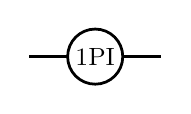
\begin{tikzpicture}[line width=1pt, scale=0.7, baseline=-0.1cm]
            \draw (-1.2,0) -- (1.2,0);
            \fill[white] (0,0) circle (0.5);
            \draw (0,0) circle (0.5);
            \node at (0,0) {\small 1PI};
        \end{tikzpicture}
    }}
    % 恒等于符号与公式
    &\equiv -i M^2(p^2) = \notag \\[1.5ex]
    % 第一项：Tadpole 蝌蚪图
    &\vcenter{\hbox{
        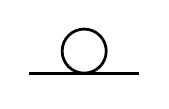
\begin{tikzpicture}[line width=1pt, scale=0.7, baseline=-0.1cm]
            \draw (-1,0) -- (1,0);
            \draw (0,0.4) circle (0.4);
        \end{tikzpicture}
    }}
    % 加号
    + 
    % 第二项：Setting-sun 日落图/气泡图
    \vcenter{\hbox{
        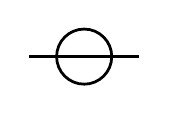
\begin{tikzpicture}[line width=1pt, scale=0.7, baseline=-0.1cm]
            \draw (-1,0) -- (1,0);
            \draw (0,0) circle (0.5);
        \end{tikzpicture}
    }}
    % 加号
    + 
    % 第三项：8字图 (Figure-8)
    \vcenter{\hbox{
        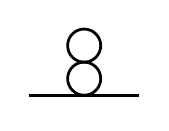
\begin{tikzpicture}[line width=1pt, scale=0.7, baseline=-0.1cm]
            \draw (-1,0) -- (1,0);
            \draw (0,0.3) circle (0.3);
            \draw (0,0.9) circle (0.3);
        \end{tikzpicture}
    }}
    % 加号与省略号
    + \cdots + \notag \\[1.5ex]
    % 第四项：反项顶点 (反项)
    &\vcenter{\hbox{
        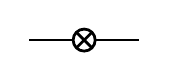
\begin{tikzpicture}[line width=1pt, scale=0.7, baseline=-0.1cm]
            \draw (-1,0) -- (1,0);
            \fill[white] (0,0) circle (0.2);
            \draw (0,0) circle (0.2);
            \draw (-0.14,-0.14) -- (0.14,0.14);
            \draw (-0.14,0.14) -- (0.14,-0.14);
        \end{tikzpicture}
    }}
    % 加号
    + 
    % 第五项：带反项顶点的蝌蚪图
    \vcenter{\hbox{
        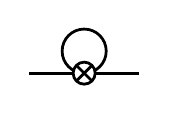
\begin{tikzpicture}[line width=1pt, scale=0.7, baseline=-0.1cm]
            \draw (-1,0) -- (1,0);
            \draw (0,0.4) circle (0.4);
            \fill[white] (0,0) circle (0.2);
            \draw (0,0) circle (0.2);
            \draw (-0.14,-0.14) -- (0.14,0.14);
            \draw (-0.14,0.14) -- (0.14,-0.14);
        \end{tikzpicture}
    }}
    % 最后的加号与省略号
    + \cdots.
\end{align}
从而我们可以将其展开为
\begin{align}
    \vcenter{\hbox{
        \begin{tikzpicture}[line width=1pt, scale=0.7, baseline=-0.1cm]
            \draw (-1.2,0) -- (1.2,0);
            \fill[white] (0,0) circle (0.3);
            \draw (0,0) circle (0.3);
            \path[pattern=north west lines] (0,0) circle (0.3);
        \end{tikzpicture}
    }}
    % 第二行开始级数展开
    &= 
    % 自由传播子 (裸线)
    \vcenter{\hbox{
        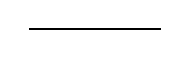
\begin{tikzpicture}[line width=1pt, scale=0.7, baseline=-0.1cm]
            \draw (-1.2,0) -- (1.2,0);
        \end{tikzpicture}
    }}
    % 加号
    + 
    % 单个 1PI 图
    \vcenter{\hbox{
        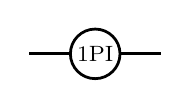
\begin{tikzpicture}[line width=1pt, scale=0.7, baseline=-0.1cm]
            \draw (-1.2,0) -- (1.2,0);
            \fill[white] (0,0) circle (0.45);
            \draw (0,0) circle (0.45);
            \node at (0,0) {\footnotesize 1PI};
        \end{tikzpicture}
    }}
    % 加号
    + 
    % 两个 1PI 串联图
    \vcenter{\hbox{
        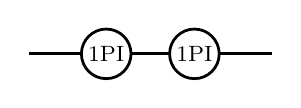
\begin{tikzpicture}[line width=1pt, scale=0.7, baseline=-0.1cm]
            \draw (-2.2,0) -- (2.2,0);
            % 第一个 1PI
            \fill[white] (-0.8,0) circle (0.45);
            \draw (-0.8,0) circle (0.45);
            \node at (-0.8,0) {\footnotesize 1PI};
            % 第二个 1PI
            \fill[white] (0.8,0) circle (0.45);
            \draw (0.8,0) circle (0.45);
            \node at (0.8,0) {\footnotesize 1PI};
        \end{tikzpicture}
    }}
    % 最后的省略号
    + \cdots.
\end{align}

这里有一点我们可能有疑惑, 就是有多个1PI串在一起的时候, 是否有内点交换的对称因子? 这是很容易想错的一个问题, 读者可能会认为这样交换内点是没有改变图的拓扑结构的, 因此$n$个1PI串在一起要贡献一个$\frac1{n!}$的因子. 但是需要注意, 所谓图的拓扑结构的定义是指交换这两个内点不改变图的邻接表, 而图的邻接表中认为每个内点都不相同: 内点的串联顺序不一样邻接表也是不一样的. 因此这里不同1PI间的内点交换改变了图的拓扑结构, 故不贡献对称因子. 于是我们知道, 
\begin{align}
    % 将整个 TikZ 图形作为一个矩阵元嵌入公式
    \vcenter{\hbox{
        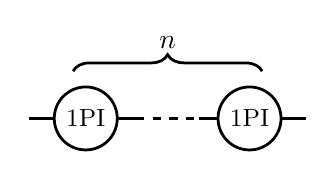
\begin{tikzpicture}[line width=1pt, scale=0.8, baseline=-0.1cm]
            % 左侧外线与第一个 1PI
            \draw (-2.2, 0) -- (-1.8, 0);
            \fill[white] (-1.3, 0) circle (0.5);
            \draw (-1.3, 0) circle (0.5);
            \node at (-1.3, 0) {\small 1PI};
            % 中间的连接线（实线 + 虚线省略 + 实线）
            \draw (-0.8, 0) -- (-0.5, 0);
            \draw[dashed, dash pattern=on 3pt off 3pt] (-0.5, 0) -- (0.5, 0);
            \draw (0.5, 0) -- (0.8, 0);
            % 最后一个 1PI 与右侧外线
            \fill[white] (1.3, 0) circle (0.5);
            \draw (1.3, 0) circle (0.5);
            \node at (1.3, 0) {\small 1PI};
            \draw (1.8, 0) -- (2.2, 0);
            % 上方的大括号与标签 n
            \draw[decorate, decoration={brace, amplitude=6pt, raise=0.2cm}] 
                (-1.5, 0.5) -- (1.5, 0.5);
            \node at (0, 1.2) {$n$};
        \end{tikzpicture}
    }}=\frac i{p^2-m^2+i\epsilon}\left(-iM^2(p^2)\frac i{p^2-m^2+i\epsilon}\right)^n
\end{align}
从而有
\begin{align}
    \vcenter{\hbox{
        \begin{tikzpicture}[line width=1pt, scale=0.7, baseline=-0.1cm]
            \draw (-1.2,0) -- (1.2,0);
            \fill[white] (0,0) circle (0.3);
            \draw (0,0) circle (0.3);
            \path[pattern=north west lines] (0,0) circle (0.3);
        \end{tikzpicture}
    }}
    % 第二行开始级数展开
    &= 
    % 自由传播子 (裸线)
    \vcenter{\hbox{
        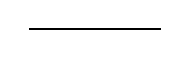
\begin{tikzpicture}[line width=1pt, scale=0.7, baseline=-0.1cm]
            \draw (-1.2,0) -- (1.2,0);
        \end{tikzpicture}
    }}
    % 加号
    + 
    % 单个 1PI 图
    \vcenter{\hbox{
        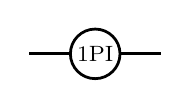
\begin{tikzpicture}[line width=1pt, scale=0.7, baseline=-0.1cm]
            \draw (-1.2,0) -- (1.2,0);
            \fill[white] (0,0) circle (0.45);
            \draw (0,0) circle (0.45);
            \node at (0,0) {\footnotesize 1PI};
        \end{tikzpicture}
    }}
    % 加号
    + 
    % 两个 1PI 串联图
    \vcenter{\hbox{
        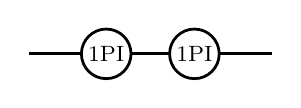
\begin{tikzpicture}[line width=1pt, scale=0.7, baseline=-0.1cm]
            \draw (-2.2,0) -- (2.2,0);
            % 第一个 1PI
            \fill[white] (-0.8,0) circle (0.45);
            \draw (-0.8,0) circle (0.45);
            \node at (-0.8,0) {\footnotesize 1PI};
            % 第二个 1PI
            \fill[white] (0.8,0) circle (0.45);
            \draw (0.8,0) circle (0.45);
            \node at (0.8,0) {\footnotesize 1PI};
        \end{tikzpicture}
    }}
    % 最后的省略号
    + \cdots\notag\\
    &=\frac i{p^2-m^2+i\epsilon}+\frac i{p^2-m^2+i\epsilon}\left(-iM^2(p^2)\right)\frac i{p^2-m^2+i\epsilon}+\cdots\notag\\
    &=\frac i{p^2-m^2-M^2(p^2)+i\epsilon}.
\end{align}

然后利用$\begin{tikzpicture}[line width=1pt]\draw (-1.2, -0.7) -- (1.2, 0.7);\draw (-1.2, 0.7) -- (1.2, -0.7);\fill[white] (0,0) circle (0.3);\draw (0,0) circle (0.3);\path[pattern=north west lines] (0,0) circle (0.3);\end{tikzpicture}$我们不难计算得到四点相互作用振幅
\begin{align}
    iM(s, t)=\begin{tikzpicture}[line width=1pt]
        \draw (-1.2, -0.7) -- (1.2, 0.7);
        \draw (-1.2, 0.7) -- (1.2, -0.7);
        \fill[white] (0,0) circle (0.3);
        \draw (0,0) circle (0.3);
        \path[pattern=north west lines] (0,0) circle (0.3);
    \end{tikzpicture}.
\end{align}

根据如上计算结果可以进行物理量的匹配. 在on-shell方案中, 极点位置为$m^2$要求
\begin{align}
    M^2(p^2)\Big|_{p^2=m^2}=0,
\end{align}
传播子的留数
\begin{align}
    \rm{Res}\left(M^2(p^2)\right)=\lim_{p^2\to m^2}\frac{i(p^2-m^2)}{p^2-m^2-M^2(p^2)+i\epsilon}=\lim_{p^2\to m^2}\frac{i}{1-\de{}{(p^2)}M^2(p^2)+i\epsilon},\notag
\end{align}
因此传播子留数为$i$要求
\begin{align}
    \de{}{(p^2)}M^2(p^2)\Big|_{p^2=m^2}=0.
\end{align}
然后考虑阈值时的散射振幅, 即两个静止的粒子经过散射仍然静止, 此时$s=(2m)^2=4m^2, t=u=0$, 得到
\begin{align}
    iM(4m^2, 0)=-i\lambda.
\end{align}
这样我们就得到了三个方程, 而我们也恰有三个反项$\delta_Z, \delta_m, \delta_\lambda$, 从而可以完全确定这三个反项, 将发散的物理量都吸收到这三者中, 实现物理量的正确匹配.

\subsubsection{利用动量截断计算圈图}
动量截断的物理意义是非常显然的: 我们的理论是低能的有效理论, 积分并不能想当然地直接推到无穷大, 我们需要引入动量截断, 控制积分收敛. 类比于Casimir效应的计算, 我们可以将高动量部分的压低抽象为引入一个带截断动量参数$\Lambda$的核函数, 从而将积分测度改为
\begin{align}
    \int\dddd p\to\int\dddd pK(p, \Lambda).
\end{align}
当然, 用来控制收敛性的核函数应当满足一定的条件, 来保证结果收敛并且物理, 总的来说有这么几个要求.
\begin{definition}[圈图积分的核函数]
    函数$K(p, \Lambda)$满足, 
    \begin{itemize}
        \item $\Lambda\to\infty$, $K(p, \Lambda)=1$,
        \item $K(p, \Lambda)$使圈图积分绝对收敛,
        \item 在IR区$p\to0$, 不引入人为的发散.
    \end{itemize}
\end{definition}
其中第二条要求可以推出
\begin{align}
    \lim_{p\to\infty}K(p, \Lambda)=0.
\end{align}

我们可以证明不同的核函数选取都不影响我们最终得到的物理结果.

上面的介绍可能略带抽象, 因此我们给出具体的计算例子来解释如何正确地匹配反项实现物理量的重匹配. 一般来说, 为了方便, 我们会直接取核函数
\begin{align}
    K(p, \Lambda)=\Theta(1-p/\Lambda).
\end{align}
这是一个硬截断, 将动量积分上限强行变为$\Lambda$.

我们计算到一阶圈图, 传播子修正(注意圈图有对称因子$2$)为
\begin{align}
    \vcenter{\hbox{
        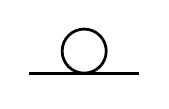
\begin{tikzpicture}[line width=1pt, scale=0.7, baseline=-0.1cm]
            \draw (-1,0) -- (1,0);
            \draw (0,0.4) circle (0.4);
        \end{tikzpicture}
    }}+\vcenter{\hbox{
        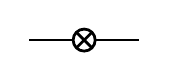
\begin{tikzpicture}[line width=1pt, scale=0.7, baseline=-0.1cm]
            \draw (-1,0) -- (1,0);
            \fill[white] (0,0) circle (0.2);
            \draw (0,0) circle (0.2);
            \draw (-0.14,-0.14) -- (0.14,0.14);
            \draw (-0.14,0.14) -- (0.14,-0.14);
        \end{tikzpicture}
    }}&=-\frac i2\lambda\int\dddd p\frac i{p^2-m^2+i\epsilon}+i(p^2\delta_Z-\delta_m).
\end{align}
考虑第一项积分, 我们很想将其分解为径向积分$\d p$与角向积分$\d\Omega$, 但是这里$p$是在双曲空间中, 而不是欧式空间中的, 这给我们做如上分解造成了困难, 因此我们需要先设法将积分转化为欧式空间中的积分. 这可以通过Wick rotation实现. 将此积分视为关于$\d p^0$的复变积分, 我们考虑如下围道.
\begin{figure}[htbp]
    \centering
    \begin{tikzpicture}[scale=2.0,
        >=Stealth,
        thick,
        decoration={markings,
            mark=at position 0.55 with {\arrow{>}}}
    ]

        % 1. 绘制标准复平面坐标轴
        \draw[->] (-1.5, 0) -- (1.5, 0) node[right] {$\text{Re}(z)$};
        \draw[->] (0, -1.5) -- (0, 1.5) node[above] {$\text{Im}(z)$};
        \node at (0, 0) [circle, fill, inner sep=1.2pt] {}; % 原点 0

        % 2. 绘制极点标记
        \node at (-1.0, 0.2) [circle, fill=black, inner sep=1.5pt, label={above:$-m+\frac i2\epsilon$}] {};
        \node at (1.0, -0.2) [circle, fill=black, inner sep=1.5pt, label={below:$m-\frac i2\epsilon$}] {};

        % --- 3. 绘制红色的非对称围道路径 (Contour Path) ---
        % 闭合路径流动顺序：原点 -> 正实轴端点 -> 第一象限弧 -> 穿过虚轴向下 -> 第三象限弧 -> 负实轴回到原点

        % 路径 1: 从原点沿着正实轴向右到 (1, 0)
        \draw[blue, postaction={decorate}] (0, 0) -- (1, 0);
        \node[blue, below] at (-0.5, 0) {$R$};

        % 路径 2: 第一象限四分之一圆弧，从 (1, 0) 到 (0, 1)
        \draw[blue, postaction={decorate}] (1, 0) arc (0:90:1.0);
        \node[blue, above right] at (0.7, 0.7) {$\Gamma_1$};

        % 路径 3: 沿虚轴垂直向下，从 (0, 1) 一直穿过原点走到 (0, -1)
        \draw[blue, postaction={decorate}] (0, 1) -- (0, -1);
        \node[blue, right] at (0, 0.5) {$I$};

        % 路径 4: 第三象限四分之一圆弧，从 (0, -1) 到 (-1, 0)
        \draw[blue, postaction={decorate}] (0, -1) arc (270:180:1.0);
        \node[blue, below left] at (-0.7, -0.7) {$\Gamma_2$};

        % 路径 5: 从左侧负实轴 (-1, 0) 向右回到原点 (0, 0) 完美闭合
        \draw[blue, postaction={decorate}] (-1, 0) -- (0, 0);
    \end{tikzpicture}
    \caption{Wick rotation}
\end{figure}

不难发现, 这个围道不包括任何极点, 因此结果为$0$. 根据大圆弧定理, 我们可以确定圆弧$\Gamma_1, \Gamma_2$的积分都为$0$, 从而
\begin{align}
    \int_R\frac{\d p^0}{2\pi}\ddd p\frac i{p^2-m^2+i\epsilon}+\int_I\frac{\d p^0}{2\pi}\ddd p\frac i{p^2-m^2+i\epsilon}=0.
\end{align}
于是实轴上从左到右的积分可以变换为虚轴上从下到上的积分, 这样$\d p^0$就是纯虚的了, 我们设
\begin{align}
    p^0=ip_E^0, 
\end{align}
则$p_E^0$就是从$-\infty$积到$+\infty$了, 并且还有
\begin{align}
    p^2=-p_E^2.
\end{align}
从而
\begin{align}
    -\frac i2\lambda\int\dddd p\frac i{p^2-m^2+i\epsilon}=-\frac i2\lambda\int i\dddd{p_E}\frac{i}{-p_E^2-m^2+i\epsilon}.
\end{align}
由此可见, 我们成功将双曲空间中的积分化为了欧式空间上的积分.

利用$n$维球面角公式, 我们不难计算得到
\begin{align}
    -\frac i2\lambda\int i\dddd{p_E}\frac{i}{-p_E^2-m^2+i\epsilon}&=-\frac{i\lambda}{32\pi^2}\int_0^{+\infty}\frac{2p_E^3\d p_E}{p_E^2+m^2},
\end{align}
我们引入动量截断$\Lambda$, 将积分上限变为$\Lambda$, 则可计算得到
\begin{align}
    -\frac i2\lambda\int i\dddd{p_E}\frac{i}{-p_E^2-m^2+i\epsilon}&=-\frac{i\lambda}{32\pi^2}\left[\Lambda^2-\ln\left(1+\frac{\Lambda^2}{m^2}\right)\right].
\end{align}

于是可以得到传播子一阶修正
\begin{align}
    M^2(p^2)=\frac\lambda{32\pi^2}\left[\Lambda^2-\ln\left(1+\Lambda^2/m^2\right)\right]-p^2\delta_Z+\delta_m.
\end{align}
利用on-shell方案的物理量匹配条件, 
\begin{align}
    &M^2(p^2)\Big|_{p^2=m^2}=0,\notag\\
    &\de{}{(p^2)}M^2(p^2)\Big|_{p^2=m^2}=0.\notag
\end{align}
我们解得
\begin{align}
    \delta_Z=0, \delta_m=-\frac\lambda{32\pi^2}\left[\Lambda^2-\ln\left(1+\Lambda^2/m^2\right)\right].
\end{align}
于是无穷大被完全抵消, 得到
\begin{align}
    M^2(p^2)=0.
\end{align}

然后计算四点关联函数的修正, 这里仅展示$s$通道, 
\begin{align}
    % --- 左侧：TikZ 绘制的费曼图 ---
    \begin{tikzpicture}[baseline=(current bounding box.center), scale=1.2]
        % 定义顶点
        \coordinate (v1) at (-0.8,0);
        \coordinate (v2) at (0.8,0);
        % 外线（输入和输出）
        \draw[thick] (-1.5, 0.7) -- (v1) node[pos=0, left] {$p_1$};
        \draw[thick] (-1.5,-0.7) -- (v1) node[pos=0, left] {$p_2$};
        \draw[thick] (v2) -- (1.5, 0.7) node[pos=1, right] {$p_3$};
        \draw[thick] (v2) -- (1.5,-0.7) node[pos=1, right] {$p_4$};
        % 圈线（Loop）
        \draw[thick] (v1) to[out=45,in=135] node[inner sep=0.5pt, label=above:$\xrightarrow{\quad k \quad}$] {} (v2);
        \draw[thick] (v1) to[out=-45,in=-135] node[inner sep=0.5pt, label=below:$\xrightarrow{\;\; p-k \;\;}$] {} (v2);
        % 总动量箭头
        \node at (-2.2, 0.1) [below] {$p = p_1 + p_2$};
        \draw[->, thick] (-2.4, 0.1) -- (-1.5, 0.1);
    \end{tikzpicture}
    % --- 中间的等号 ---
    &=\frac{(-i\lambda)^2}{2} \int\dddd p \frac{i}{k^2 - m^2 + i\epsilon} \frac{i}{(p-k)^2 - m^2 + i\epsilon}.
\end{align}
需要注意, 这里有顶点内置换产生的对称因子$2$. 利用附录定理\ref{feynman-trick}中的Feynman's Trick可以得到
\begin{align}
    &=\frac{\lambda^2}2\int\dddd k\int_0^1\dx\frac1{\left[k^2-m^2+i\epsilon+x(p^2-2p\cdot k)\right]^2},
\end{align}
然后配方, 并换元$k-px\to k$, 可得
\begin{align}
    &=\frac{\lambda^2}2\int_0^1\dx\int\dddd k\frac1{\left[(k-px)^2+p^2x(1-x)-m^2+i\epsilon\right]^2}\notag\\
    &=\frac{\lambda^2}2\int_0^1\dx\int\dddd k\frac1{\left[k^2+p^2x(1-x)-m^2+i\epsilon\right]^2}, 
\end{align}
做Wick rotation可以得到
\begin{align}
    &=\frac{i\lambda^2}2\int_0^1\dx\int\dddd{k_E}\frac1{\left[-k_E^2+p^2x(1-x)-m^2+i\epsilon\right]^2}
\end{align}
设$\Delta(s=p^2)=m^2-sx(1-x)-i\epsilon$, 并先后积掉角向与径向, 可以得到
\begin{align}
    &=\frac{i\lambda^2}{32\pi^2}\int_0^1\dx\left[\ln\frac{\Delta+\Lambda^2}{\Delta}-\frac{\Lambda^2}{\Lambda^2+\Delta}\right].
\end{align}

类似地加上$t, u$通道, 则可以得到修正后的四点关联函数
\begin{align}
    iM=\begin{tikzpicture}[line width=1pt]
        \draw (-1.2, -0.7) -- (1.2, 0.7);
        \draw (-1.2, 0.7) -- (1.2, -0.7);
        \fill[white] (0,0) circle (0.3);
        \draw (0,0) circle (0.3);
        \path[pattern=north west lines] (0,0) circle (0.3);
    \end{tikzpicture}=-i\lambda+\sum_{c=s,t,u}\frac{i\lambda^2}{32\pi^2}\int_0^1\dx\left[\ln\frac{\Delta(c)+\Lambda^2}{\Delta}-\frac{\Lambda^2}{\Lambda^2+\Delta(c)}\right]-i\delta_\lambda.
\end{align}

利用$iM(s=4m^2, t=u=0)=-i\lambda$, 设$\Delta_0(c)=m^2-c_0x(1-x)-i\epsilon$, 其中$c=s, t, u$, 而$s_0=4m^2, t_0=u_0=0$, 我们可以解得反项
\begin{align}
    \delta_\lambda=\frac{\lambda^2}{32\pi^2}\sum_{c=s,t,u}\int_0^1\dx\left[\ln\frac{\Delta_0(c)+\Lambda^2}{\Delta_0(c)}-\frac{\Lambda^2}{\Lambda^2+\Delta_0(c)}\right],
\end{align}

从而有修正一阶修正的四点关联函数
\begin{align}
    iM=-i\lambda+\frac{i\lambda^2}{32\pi^2}\sum_{c=s,t,u}\int_0^1\dx\left[\ln\frac{\Delta(c)+\Lambda^2}{\Delta_0(c)+\Lambda^2}\frac{\Delta_0(c)}{\Delta(c)}-\frac{\Lambda^2}{\Lambda^2+\Delta(c)}+\frac{\Lambda^2}{\Lambda^2+\Delta_0(c)}\right].
\end{align}
可以发现, 现在无穷大就已经全部被吸收掉了, 取$\Lambda\to\infty$仍然可以保证关联函数是有限的. 于是我们直接计算$\Lambda\to\infty$后的极限, 得到
\begin{align}
    iM&=-i\lambda-\frac{i\lambda^2}{32\pi^2}\sum_{c=s,t,u}\int_0^1\dx\ln\frac{\Delta(c)}{\Delta_0(c)}\notag\\
    &=-i\lambda-\frac{i\lambda^2}{32\pi^2}\sum_{c=s,t,u}\int_0^1\dx\ln\frac{m^2-cx(1-x)-i\epsilon}{m^2-c_0x(1-x)-i\epsilon}.
\end{align}
利用分部积分, 经过艰苦卓绝的爆算我们可以得到
\begin{align}
    \int_0^1\dx\ln\left(m^2-cx(1-x)-i\epsilon\right)&=\ln m^2-2+2\sqrt{\frac{4m^2}{c}-1-i\epsilon}\arctan\frac1{\sqrt{\frac{4m^2}{c}-1-i\epsilon}},
\end{align}
设辅助函数
\begin{align}
    A(c)=\sqrt{\frac{4m^2}{c}-1-i\epsilon}\arctan\frac1{\sqrt{\frac{4m^2}{c}-1-i\epsilon}}
\end{align}
在这里保留$i\epsilon$是因为当碰撞高于阈值$s>4m^2$时, $\sqrt{\frac{4m^2}{s}-1}$为纯虚的, 而$i\epsilon$则可以挑选出我们需要的分支. 从而有
\begin{align}
    iM&=-i\lambda-\frac{i\lambda^2}{16\pi^2}\left[A(s)+A(u)+A(t)-A(4m^2)-2A(0)\right].
\end{align}
而$A(4m^2)=0, A(0)=1$, 于是最终可得
\begin{align}
    M(s, t, u)&=-\lambda-\frac{\lambda^2}{16\pi^2}\left[(A(s)+A(u)+A(t)-2)\right].
\end{align}

\subsubsection{利用维数调控计算圈图}
动量截断非常物理也非常直接, 在处理$\phi^4$场论的时候非常好用, 但是涉及到规范场则会显得有些力不从心: 一个强行的动量截断显然破坏了Lorentz对称性与规范对称性. 一个优雅的解决方案是使用维数调控: 假设我们并不是在$d=4$维考虑量子场论, 而是在$d=4-2\epsilon$考虑.

读者可能会疑惑, 维度调控的引入到底是为什么, 它的物理意义是什么. 笔者认为, 这其实只是引入了一种特殊的核函数来进行动量截断, 但其特殊之处就在于不是以某一个物理的截断动量$\Lambda$为核的参数, 而是以一个表示维度的无量纲$\epsilon$(一般地来说可以为复)为参数, 
\begin{align}
    K_D(p, \epsilon)=\frac{\Gamma(2)}{\Gamma(2-\epsilon)}\pi^{-\epsilon}\mu^{2\epsilon}p^{-2\epsilon}.
\end{align}
其中$\mu$是一任意的动量量纲的常数, 是用来控制量纲使得核函数无量纲的. 而前面奇怪的$\Gamma$与$\pi$组成的系数只是为了凑$4-2\epsilon$维的球面角.

这样的好处在于, 无论是多少次的发散积分, 只要我们$\epsilon$取的实部足够大, 都可以得到一个收敛的积分. 得到结果后, 再利用复平面上的解析延拓, 我们可以让这个积分结果在复平面上除孤立极点外都收敛, 从而成功推到$\epsilon\to0$的区域. 后面的计算告诉我们, 可以预料在$\epsilon=0$处是一个一阶极点, 也就是所有的发散都被吸收到了$\frac1\epsilon$中.

我们用维数调控再次计算上节的结果.
\begin{align}
    \vcenter{\hbox{
        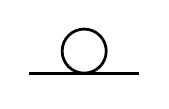
\begin{tikzpicture}[line width=1pt, scale=0.7, baseline=-0.1cm]
            \draw (-1,0) -- (1,0);
            \draw (0,0.4) circle (0.4);
        \end{tikzpicture}
    }}&=-\frac{i\lambda}2\mu^{2\epsilon}\int\nd d p\frac i{p^2-m^2+i\epsilon}\\
    &=-\frac{i\lambda}{2}\frac{\mu^{2\epsilon}}{(4\pi)^{d/2}}\frac{\Gamma(1-\frac d2)}{(m^2)^{1-d/2}}\\
    &=\frac{i\lambda m^2}{32\pi^2}\left(\frac1\epsilon-\gamma+1+\ln(4\pi)-\ln\frac{m^2}{\mu^2}\right).
\end{align}
不难注意到, 确实如我们所预料的, 所有的无穷大量都体现在$\frac1\epsilon$中.

利用on-shell方案的条件可以得到
\begin{align}
    \delta_Z=0, \delta_m=-\frac{\lambda}{2}\frac{\mu^{2\epsilon}}{(4\pi)^{d/2}}\frac{\Gamma(1-\frac d2)}{(m^2)^{1-d/2}}.
\end{align}
同样有
\begin{align}
    M^2(p^2)=0.
\end{align}

然后计算四点关联函数
\begin{align}
    % --- 左侧：TikZ 绘制的费曼图 ---
    \begin{tikzpicture}[baseline=(current bounding box.center), scale=1.2]
        % 定义顶点
        \coordinate (v1) at (-0.8,0);
        \coordinate (v2) at (0.8,0);
        % 外线（输入和输出）
        \draw[thick] (-1.5, 0.7) -- (v1) node[pos=0, left] {$p_1$};
        \draw[thick] (-1.5,-0.7) -- (v1) node[pos=0, left] {$p_2$};
        \draw[thick] (v2) -- (1.5, 0.7) node[pos=1, right] {$p_3$};
        \draw[thick] (v2) -- (1.5,-0.7) node[pos=1, right] {$p_4$};
        % 圈线（Loop）
        \draw[thick] (v1) to[out=45,in=135] node[inner sep=0.5pt, label=above:$\xrightarrow{\quad k \quad}$] {} (v2);
        \draw[thick] (v1) to[out=-45,in=-135] node[inner sep=0.5pt, label=below:$\xrightarrow{\;\; p-k \;\;}$] {} (v2);
        % 总动量箭头
        \node at (-2.2, 0.1) [below] {$p = p_1 + p_2$};
        \draw[->, thick] (-2.4, 0.1) -- (-1.5, 0.1);
    \end{tikzpicture}
    % --- 中间的等号 ---
    &=\frac{(-i\lambda)^2}{2}\int\mu^{2\epsilon}\nd dp \frac{i}{k^2 - m^2 + i\epsilon} \frac{i}{(p-k)^2 - m^2 + i\epsilon}.
\end{align}
利用Feynman's Trick与附录\ref{dim-reg-loop-refer}, 可以得到
\begin{align}
    &=\frac{i\lambda^2}{2}\mu^{2\epsilon}\int_0^1\dx\frac{\Gamma(\epsilon)}{(4\pi)^{d/2}}\frac1{\Delta^\epsilon}\\
    &=\frac{i\lambda^2}{32\pi^2}\int_0^1\dx\left(\frac1\epsilon-\gamma+\ln4\pi-\ln\frac{m^2-p^2x(1-x)-i\epsilon}{\mu^2}\right).
\end{align}
后面的计算是类似的, 解出
\begin{align}
    \delta_\lambda=\sum_{c=s, t, u}\frac{\lambda^2}{32\pi^2}\int_0^1\dx\left(\frac1\epsilon-\gamma+\ln4\pi-\ln\frac{m^2-c_0x(1-x)-i\epsilon}{\mu^2}\right),
\end{align}
即可得到同样的散射振幅
\begin{align}
    M(s, t, u)&=-\lambda-\frac{\lambda^2}{16\pi^2}\left[(A(s)+A(u)+A(t)-2)\right].
\end{align}
这也从侧面印证了维数调控的正确性.

\subsubsection{MS、$\overline{MS}$方案与重整化群流}
on-shell方案很清楚也很物理, 但是缺点在于随着圈数提高, 满足它的on-shell条件会越来越麻烦; 其次, 有些时候它计算出来的结果在特殊情况下会有奇异性. 比如上一节计算出来的$\phi^4$一阶修正中, 取$m\to0$就会导致奇异性, 这就是红外发散. 为了能够正确处理无质量粒子, 并且简化计算, 我们实际更常用的是MS或者$\overline{MS}$方案. 所谓的MS其实是Minimal Substraction的缩写. 

继续以$\phi^4$理论为例, 在维数调控中, 我们计算出结果
\begin{align}
    \vcenter{\hbox{
        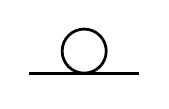
\begin{tikzpicture}[line width=1pt, scale=0.7, baseline=-0.1cm]
            \draw (-1,0) -- (1,0);
            \draw (0,0.4) circle (0.4);
        \end{tikzpicture}
    }}&=\frac{i\lambda m^2}{32\pi^2}\left(\frac1\epsilon-\gamma+1+\ln4\pi-\ln\frac{m^2}{\mu^2}\right),\notag
\end{align}
\begin{align}
    % --- 左侧：TikZ 绘制的费曼图 ---
    \begin{tikzpicture}[baseline=(current bounding box.center), scale=1.2]
        % 定义顶点
        \coordinate (v1) at (-0.8,0);
        \coordinate (v2) at (0.8,0);
        % 外线（输入和输出）
        \draw[thick] (-1.5, 0.7) -- (v1) node[pos=0, left] {$p_1$};
        \draw[thick] (-1.5,-0.7) -- (v1) node[pos=0, left] {$p_2$};
        \draw[thick] (v2) -- (1.5, 0.7) node[pos=1, right] {$p_3$};
        \draw[thick] (v2) -- (1.5,-0.7) node[pos=1, right] {$p_4$};
        % 圈线（Loop）
        \draw[thick] (v1) to[out=45,in=135] node[inner sep=0.5pt, label=above:$\xrightarrow{\quad k \quad}$] {} (v2);
        \draw[thick] (v1) to[out=-45,in=-135] node[inner sep=0.5pt, label=below:$\xrightarrow{\;\; p-k \;\;}$] {} (v2);
    \end{tikzpicture}
    &=\frac{i\lambda^2}{32\pi^2}\int_0^1\dx\left(\frac1\epsilon-\gamma+\ln4\pi-\ln\frac{m^2-p^2x(1-x)-i\epsilon}{\mu^2}\right).\notag
\end{align}
然后即可给出这两种方案的定义.
\begin{definition}[MS方案]
    MS方案就是指通过维度调控计算圈图, 反项仅抵消极点$\frac1\epsilon$.
\end{definition}
更方便的选择则是把$\frac1\epsilon$后面的无关常数$\gamma, \ln4\pi$等也一起吸收到反项中, 这被称为$\overline{MS}$方案.
\begin{definition}[$\overline{MS}$方案]
    $\overline{MS}$方案就是指通过维度调控计算圈图, 反项抵消极点$\frac1\epsilon$与无关系数$\gamma, \ln4\pi$等.
\end{definition}

我们一般直接使用$\overline{MS}$方案. 也就是
\begin{align}
    & \delta_Z=0,\notag\\
    & \delta_m=\frac{\lambda m^2}{32\pi^2}\left(\frac1\epsilon-\gamma+\ln4\pi\right),\\
    & \delta_\lambda=\frac{3\lambda^2}{32\pi^2}\left(\frac1\epsilon-\gamma+\ln4\pi\right).
\end{align}
这里只需要注意因为$\delta_\lambda$需要一次性扣掉$s, t, u$三个通道的发散, 因此前面多了一个因子$3$. 于是可得
\begin{align}
    & M^2(p^2)=\frac{\lambda m^2}{32\pi^2}\left(\ln\frac{m^2}{\mu^2}-1\right),\\
    & iM=-i\lambda-\frac{i\lambda^2}{32\pi^2}\sum_{c=s,t,u}\int_0^1\dx\ln\frac{m^2-cx(1-x)-i\epsilon}{\mu^2}.
\end{align}

需要注意, 与on-shell方案, 现在加入反项后的Lagrangian里面的参数$m, \lambda$也已经不代表真实的物理量了. 设真实的物理质量为$m_P$, 则
\begin{align}
    m_p^2=m^2+M^2(p^2)=m^2+\frac{\lambda m^2}{32\pi^2}\left(\ln\frac{m^2}{\mu^2}-1\right).
\end{align}
散射振幅为
\begin{align}
    M(s, t, u)=-\lambda-\frac{\lambda^2}{16\pi^2}\left[A(s)+A(t)+A(u)-3+\frac32\ln\frac{m^2}{\mu^2}\right].
\end{align}

这里存在一个诡异的问题: 为什么计算出来的物理量会依赖于一个纯粹人为引入的参数$\mu$, 这个计算结果是否可信? 原因在此, 我们还没有制定$m$, $\lambda$具体的值: 不同于on-shell方案, 我们并没有给它们指定与任何物理实际参数相关. 只要$m, \lambda$是关于$\mu$的函数, 将非物理的依赖$\mu$完全吸收到$m, \lambda$内部即可. 要求$m, \lambda$关于$\mu$的方程, 可以利用物理态与$\mu$无关的性质:
\begin{align}
    \de{}{\mu}m_P=0, \de{}{\mu}M=0.
\end{align}
从第一个方程可得
\begin{align}
    0=\de{m^2}{\mu}\left(1+\frac\lambda{32\pi^2}\ln\frac{m^2}{\mu^2}\right)-\frac{\lambda m^2}{16\pi^2}\frac1\mu+\frac{m^2}{32\pi^2}\left(\ln\frac{m^2}{\mu^2}-1\right)\de\lambda\mu.
\end{align}
然后注意到, 我们的微扰论精度只到一阶精度, $\mu\de{m^2}\mu\sim\lambda$, $\mu\de\lambda\mu\sim\lambda^2$, 因此我们可以将所有高于预计一阶的项都忽略, 从而得到
\begin{align}
    \mu\de{m^2}\mu=\frac{\lambda m^2}{16\pi^2}.\label{phi4-1loop-rg-m}
\end{align}
类似地有
\begin{align}
    \mu\de\lambda\mu=\frac{3\lambda^2}{16\pi^2}.\label{phi4-1loop-rg-lambda}
\end{align}
如上两个方程\eqref{phi4-1loop-rg-m}, \eqref{phi4-1loop-rg-lambda}就是重整化群方程(RG Equation).

不过一般来说我们更希望重整化群方程中的$m, \lambda$是无量纲化的, 因此不妨设
\begin{align}
    \widetilde m^2=\frac{m^2}{\mu^2},
\end{align}
从而有
\begin{align}
    & \mu\de{\widetilde m^2}\mu=\frac{\lambda\widetilde m^2}{16\pi^2}-2\widetilde m^2,\\
    & \mu\de\lambda\mu=\frac{3\lambda^2}{16\pi^2}.\notag
\end{align}
根据重整化群方程, 我们可以画出参数空间$\widetilde m^2, \lambda$中, 两参数随能标$\mu$增大的流向, 也就是重整化群流, 如图\ref{phi4-1loop-rgf}.
\begin{figure}[!htbp]
    \centering
    
\includegraphics[page=1,width=0.4\textwidth]{phi4-1loop-rgf.pdf}
    \caption{$\phi^4$重整化群流}\label{phi4-1loop-rgf}
\end{figure}

\subsubsection{什么是不可重整化?}
对于$\Delta_i\geq0$, 积分产生无穷大的根源是我们没有正确地匹配物理量与观测结果: 只要我们正确地将实验观测量与物理量进行匹配, 即可得到具有预测能力的物理理论. 但是对于$\Delta_i<0$的理论, 情况就糟糕很多了: 我们有无穷多个振幅(子图)是发散的, 这意味着我们需要引入无穷多个反项, 并与无穷多个实验测量结果进行拼配: 这使得我们的理论完全失去了预言能力. 读者可能会疑惑, 我们不是总共就这么几个参数吗, 为什么需要引入无穷多个反项. 这里我们做进一步的讨论, 考虑一个$\phi^6$理论
\begin{align}
    \mathcal L=\frac12(\partial\phi)^2-\frac12m^2\phi^2-\frac\lambda{6!}\phi^6,
\end{align}
我们不难首先得到反项
\begin{align}
    \mathcal L=\frac12(\partial\phi_r)^2-\frac12 m^2\phi_r^2-\frac\lambda{6!}\phi_r^6+\frac12\delta_Z(\partial\phi_r)^2-\frac12\delta_m\phi^2-\frac{\delta_\lambda}{6!}\phi_r^6,
\end{align}
这看起来没啥问题, 如果使用on-shell方案, 我们只需要继续让$\delta_Z, \delta_m, \delta_\lambda$与实验观测结果匹配即可. 但是问题在于, 随着我们考虑更多顶点, 会出现我们原有反项无法消除的无穷大, 这需要我们凭空在Lagrangian里面引入新的反项来抵消无穷大, 最终引入无穷多个反项以至于理论完全失去预言能力.

从现代观点来看, 我们认为不可重整化理论只是更高能理论的一个低能有效场论. 我们由于实验技术限制, 只能在低能尺度$E$($E\ll M$, 其中$M$为某个特征能标, $\lambda_6\propto\frac1{M^2}$). 做实验时，那些高能的未知动力学(比如复杂的弦振动、或者未知的重粒子交换)在我们看来，就被凝聚/积掉(Integrated out)成了低能Lagrangian里的非线性接触项(即$\phi^6, \phi^8\dots$, 并且这些非线性项是被我们高能理论极大的能标$M$给强烈压制的). 此时, $\lambda_6$的物理大小其实是由高能理论决定的, 它天然地正比于$\frac{1}{M^2}$. 而作为一个低能有效理论, 我们本来就不应该把动量积到无穷大, 而是在动量到$M$附近就停止了, 这就是动量截断的物理意义. 

\subsection{旋量QED的重整化}
\subsubsection{真空极化}
考虑光子传播子的单圈修正
\begin{align}
    \begin{tikzpicture}[baseline=(current bounding box.center)]
        \begin{feynman}
            \diagram* {
                a -- [photon] b -- [fermion, half left] c -- [photon] d,
                c -- [fermion, half left] b,
            };
        \end{feynman}
    \end{tikzpicture}=-(-ie)^2\int&\dddd p\frac{i}{(p-k)^2-m^2+i\epsilon}\frac{i}{k^2-m^2+i\epsilon}\notag\\
    &\;\;\rm{Tr}\left(\gamma^\mu(\slashed k-\slashed p+m)\gamma^\nu(\slashed p+m)\right)
\end{align}
经过计算可得
\begin{align}
    \mathcal M_{\mu\nu}=-\frac{e^2p^2}{12\pi^2}g_{\mu\nu}\left(\frac2\epsilon+\frac16\ln\frac{\mu^2}{-p^2}+\frac5{18}\right)
\end{align}
其中
\begin{equation}
    \ln\mu^2=\ln(4\pi)-\gamma.
\end{equation}

% 所以我们可以计算得到光子传播子的一圈修正为
% \begin{equation}
    
% \end{equation}